\documentclass[a4paper,12pt]{article}
\usepackage[english,ukrainian,russian]{babel}
\linespread{1}
\usepackage{ucs}
\usepackage[utf8]{inputenc}
\usepackage[T2A]{fontenc}
\usepackage[paper=portrait,pagesize]{typearea}
\usepackage{amsmath}
\usepackage{bigints}
\usepackage{amsfonts}
\usepackage{graphicx}
\usepackage{amssymb}
\usepackage{cancel}
\usepackage{gensymb}
\usepackage{multirow}
\usepackage{rotate} 
\usepackage{pdflscape}
\usepackage{bigstrut}
\usepackage[pageanchor]{hyperref}
\usepackage{chngpage}
\newcommand{\dx}{\textbf{d}x}
\newcommand{\dt}{\textbf{d}t}
\newcommand{\du}{\textbf{d}u}
\newcommand{\dv}{\textbf{d}v}
\newcommand{\dy}{\textbf{d}y}
\newcommand{\ds}{\textbf{d}s}
\newcommand{\dz}{\textbf{d}z}
\newcommand{\arch}{\textrm{arcch}}
\newcommand{\arsh}{\textrm{arcsh}}
\newcommand{\dint}{\displaystyle\int}
\newcommand\tab[1][1cm]{\hspace*{#1}}
\newcommand{\RomanNumeralCaps}[1]{\MakeUppercase{\romannumeral #1}}
\newcommand{\dsum}{\displaystyle\sum}
\usepackage[left=20mm, top=20mm, right=15mm, bottom=15mm, nohead, nofoot]{geometry}
\usepackage{verbatim}
\usepackage{enumerate}
\usepackage{listings}
\usepackage{xcolor}

\definecolor{codegreen}{rgb}{0,0.6,0}
\definecolor{codegray}{rgb}{0.5,0.5,0.5}
\definecolor{codepurple}{rgb}{0.58,0,0.82}
\definecolor{backcolour}{rgb}{0.95,0.95,0.92}

\lstdefinestyle{mystyle}{
	backgroundcolor=\color{backcolour},   
	commentstyle=\color{codegreen},
	keywordstyle=\color{blue},
	numberstyle=\tiny\color{codegray},
	stringstyle=\color{red},
	basicstyle=\ttfamily\footnotesize,
	breakatwhitespace=false,         
	breaklines=true,                 
	captionpos=b,                    
	keepspaces=true,                 
	numbers=none,                    
	numbersep=5pt,                  
	showspaces=false,                
	showstringspaces=false,
	showtabs=false,                  
	tabsize=4,
	frame=shadowbox
}

\lstset{style=mystyle}


\begin{document}
	\begin{center}
		{\Large \bfseries \textsc{Лабораторна робота №9}}\\
		\hrulefill\\
		\Large \textsc{ФІ-12 Завалій Олександр\\ Варіант №5}
	\end{center}
	\begin{center}
		\section*{\bfseries{Завдання}}
	\end{center} 
	\textbf{Предметна область:} \\
	Навчально-методичне управління (облік площі приміщень). \\
	\textbf{Основні предметно-значущі сутності:} \\
	Приміщення, Підрозділи. \\
	\textbf{Основні предметно-значущі атрибути сутностей:}
	\begin{enumerate}
		\item[-] \textbf{Приміщення}: назва або номер приміщення, вид приміщення (аудиторія, кабінет і т.п.), площа, кількість посадочних місць, підрозділ. 
		\item[-] \textbf{Підрозділи}: назва, вид підрозділу.
	\end{enumerate}
	\textbf{Основні вимоги до функцій системи:}
	\begin{enumerate}
		\item[-] Вибрати назви або номери приміщень за підрозділами;
		\item[-] Підрахувати загальну площу навчальних аудиторій по приміщеннях і в цілому по навчальному закладу;
		\item[-] Підрахувати загальну кількість посадочних місць для співробітників по підрозділам.
	\end{enumerate}
	\textbf{Тригери:}
	\begin{enumerate}
		\item На видалення запису з таблиці «Приміщення». Якщо для приміщення зазначено підрозділ, заборонити видалення запису.
		\item Створити представлення «Аудиторії» з полями «код приміщення», «назва приміщення», «підрозділ», в яку повинні входити приміщення виду «Аудиторія». Оновлювати представлення «Аудиторії».
	\end{enumerate}
	\textbf{Процедура:}\\
	Процедура повинна повертати кількість приміщень для зазначеного підрозділу. \\

\newpage
	\begin{center}
		\section*{\bfseries{Реалізація завдання}}
	\end{center}
    \begin{center}
        \Large{Task \RomanNumeralCaps{1}}
    \end{center}
	\textbf{\RomanNumeralCaps{1}.\RomanNumeralCaps{1}}
	Створити новий обліковий запис.
	\begin{lstlisting}[language=SQL]
	USE TestProject
	GO
	
	CREATE LOGIN Bill_Login
	WITH PASSWORD='password',
	DEFAULT_DATABASE=TestProject;
	GO
	
	CREATE USER Bill FOR LOGIN Bill_Login
	GO
	\end{lstlisting}

	\textbf{\RomanNumeralCaps{1}.\RomanNumeralCaps{2}}
	Назначити користувачу роль БД.
	\begin{lstlisting}[language=SQL]
	CREATE SERVER ROLE TableAdmin 
	GO  

	ALTER SERVER ROLE TableAdmin ADD MEMBER Bill_Login
	GO 
	\end{lstlisting}

	\textbf{\RomanNumeralCaps{1}.\RomanNumeralCaps{3}}
	Надати користувачу Bill повноваження на доступ к збереженої процедури.
	\begin{lstlisting}[language=SQL]
	GRANT EXECUTE ON OBJECT::AmountOfRoom  
		TO Bill
	GO
	\end{lstlisting}

	\textbf{\RomanNumeralCaps{1}.\RomanNumeralCaps{4}}
	Відкликати всі надані користувачу Bill привілегії.
	\begin{lstlisting}[language=SQL]
	REVOKE EXECUTE ON OBJECT::AmountOfRoom TO Bill
	GO
	
	ALTER SERVER ROLE TableAdmin DROP MEMBER Bill_Login
	\end{lstlisting}

\newpage
    \begin{center}
        \Large{Task \RomanNumeralCaps{2}}
    \end{center}
	\begin{center}
		\textbf{Поясніть призначення команд Transact SQL.}
	\end{center}
	\begin{enumerate}
		\item[$a)$] Надаємо дозвіли <<SELECT>> та <<INSERT>> користувачу <<J\_Smith>> на таблицю <<SUPPLIES>> 
		з можливістю надати ці дозволи іншим об'єктам. Користувач <<Economists>> надає дозвіл 
		користувачу <<J\_Smith>> на успадкування цих можливостей.
		\item[$b)$] У наступному прикладі створюється SQL Server login для 
		користувача <<king\_of\_the\_db>> із паролем <<a2h7d0f7dg84mdf94>>, з базою даних за 
		замовчуванням <<PROJECTS>>, мовою за замовчуванням <<Ukrainian>>, ідентифікатором безпеки (sid)
		<<master>>, та пароль передається у відкритому вигляди. Тобто ніяк не шифрується.
		\item[$c)$] Відміняємо всі надані привілеї користувачу <<M\_Ivanenko>>.
		Параметр <<CASCADE>> вказує на те, що дозвіл також скасовується і в користувачів, які отримали доступ через цього користувача.
	\end{enumerate}

	\begin{center}
        \Large{Task \RomanNumeralCaps{3}}
    \end{center}
	\begin{center}
		\textbf{Зашифруйте зміст однієї з колонок таблиці в створеній БД.}
	\end{center}
	\begin{lstlisting}[language=SQL]
	USE master;
	GO
	SELECT *
	FROM sys.symmetric_keys
	WHERE name = '##MS_ServiceMasterKey##';
	GO
	
	USE TestProject;
	GO
	CREATE MASTER KEY ENCRYPTION BY PASSWORD = 'password';
	GO
	
	CREATE CERTIFICATE Certificate1
	WITH SUBJECT = 'Protect Data';
	GO
	
	CREATE SYMMETRIC KEY SymmetricKey1 
	WITH ALGORITHM = AES_128 
	ENCRYPTION BY CERTIFICATE Certificate1;
	GO
	
	ALTER TABLE dbo.Ownerss 
	ADD first_name_encrypt varbinary(MAX) NULL
	GO
	
	USE TestProject;
	GO
	OPEN SYMMETRIC KEY SymmetricKey1
	DECRYPTION BY CERTIFICATE Certificate1;
	GO
	UPDATE dbo.Ownerss
	SET first_name_encrypt = EncryptByKey 
	(Key_GUID('SymmetricKey1'), FirstName)
	FROM dbo.Ownerss;
	GO
	CLOSE SYMMETRIC KEY SymmetricKey1;
	GO
	\end{lstlisting}

\newpage
	\begin{lstlisting}[language=SQL]
	USE TestProject;
	GO
	ALTER TABLE dbo.Ownerss
	DROP COLUMN FirstName;
	GO
	
	SELECT *
	FROM dbo.Ownerss
	GO
	\end{lstlisting}
	\begin{figure}[h!]
		\begin{minipage}[h]{1\linewidth}
			\centering
			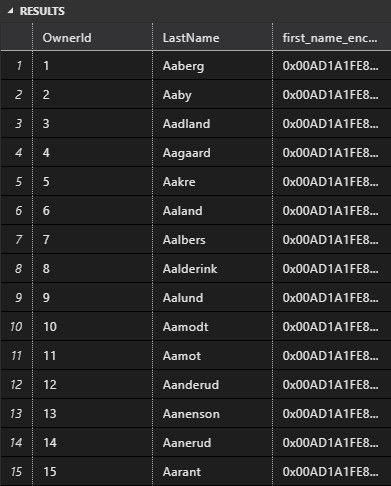
\includegraphics[width=0.5\linewidth]{Prt sc/Figure_1.jpg}  
		\end{minipage}
		\caption{Таблиця <<dbo.Ownerss>> з зашифрованими даними.}
	\end{figure}
	\begin{lstlisting}[language=SQL]
	USE TestProject
	GO
	OPEN SYMMETRIC KEY SymmetricKey1
	DECRYPTION BY CERTIFICATE Certificate1;
	GO
	SELECT 
	CONVERT(varchar, DecryptByKey(first_name_encrypt)) 
	AS 'Decrypted first name', LastName
	FROM dbo.Ownerss;
	CLOSE SYMMETRIC KEY SymmetricKey1;
	GO
	\end{lstlisting}
	\begin{figure}[h!]
		\begin{minipage}[h]{1\linewidth}
			\centering
			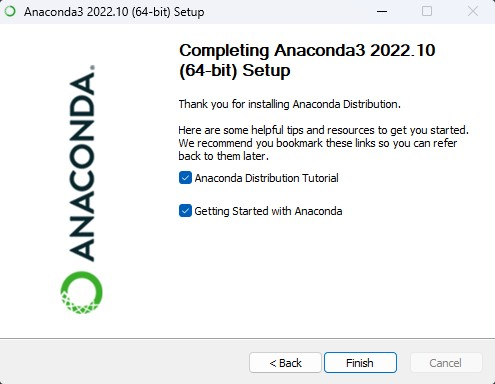
\includegraphics[width=0.5\linewidth]{Prt sc/Figure_2.jpg}  
		\end{minipage}
		\caption{Переглядаємо зашифровані дані.}
	\end{figure}
	
\end{document}